\documentclass[sigconf,nonacm]{acmart}

%%
%% Packages for diagrams and charts
\usepackage{tikz}
\usepackage{pgfplots}
\usepackage{pgfplotstable}
\pgfplotsset{compat=1.18}
\usetikzlibrary{shapes,arrows,positioning,fit,backgrounds,calc}

%%
%% \BibTeX command to typeset BibTeX logo in the docs
\AtBeginDocument{%
  \providecommand\BibTeX{{%
    Bib\TeX}}}

%% Rights management information.
\copyrightyear{2026}
\acmYear{2026}
\setcopyright{acmlicensed}
\acmConference[MLSys'26]{Conference on Machine Learning and Systems}{March 2026}{Palo Alto, CA, USA}

%%
%% These commands are for a PROCEEDINGS abstract or paper.
\acmBooktitle{Conference Proceedings on Machine Learning and Systems}
\acmPrice{15.00}
\acmDOI{10.1145/XXXXXX.XXXXXX}
\acmISBN{978-1-4503-XXXX-X/26/03}

%%
%% end of the preamble, start of the body of the document source.
\begin{document}

%%
%% The "title" command has an optional parameter,
%% allowing the author to define a "short title" to be used in page headers.
\title{Arena: A Rigorous Benchmarking Framework for Evaluating Production-Ready LLM Agent Systems}

%%
%% The "author" command and its associated commands are used to define
%% the authors and their affiliations.
\author{Roberto Milev}
\email{rmilev@navan.com}
\affiliation{%
  \institution{Navan}
  \city{Palo Alto}
  \state{CA}
  \country{USA}
}

\author{Uday Bhanu Prasad Kanagala}
\email{ukanagala@navan.com}
\affiliation{%
  \institution{Navan}
  \city{Palo Alto}
  \state{CA}
  \country{USA}
}

%%
%% The abstract is a short summary of the work to be presented in the
%% article.
\begin{abstract}
The proliferation of Large Language Model (LLM)-based agent frameworks has created significant challenges for practitioners in selecting optimal systems for production deployment. Despite the critical importance of this decision, existing benchmarking methodologies suffer from three fundamental limitations: (1) evaluation of base models rather than complete agent frameworks with tool integration, (2) reliance on synthetic tasks rather than production-realistic scenarios, and (3) sequential testing that introduces systematic position bias through caching and API throttling effects.

We present \textbf{Arena}, a comprehensive benchmarking framework that addresses these limitations through rigorous experimental design and novel parallel execution methodology. Arena evaluates four production-ready agent frameworks—Claude SDK, Google ADK, AWS Strands, and CrewAI—on AWS Bedrock using Claude Sonnet 4.5 across 204 benchmark runs spanning 7 iterations. We assess performance along seven dimensions: correctness (0-100\%), latency, consistency, token efficiency, step efficiency, code complexity, and cost-effectiveness.

Our empirical investigation reveals three critical insights: (1) framework performance rankings exhibit complete reversal between simple scenarios (3-4 steps) and complex scenarios (8 steps), with Google ADK demonstrating 36\% degradation (92\%→58\%) while Claude SDK maintains robustness with only 10\% degradation (92\%→82\%); (2) sequential testing introduces statistically significant position-dependent bias (20\%+ latency variance, p<0.001), validating parallel execution as methodologically essential; and (3) temperature=0 enables reproducible evaluation with 0\% variance for 50\% of frameworks and <2\% variance for all frameworks tested.

Claude SDK emerges as the definitive choice for production deployments, achieving 88.58\% correctness with perfect 100\% consistency and 0\% variance across iterations, while maintaining superior cost-effectiveness (\$0.038/run versus \$0.091/run for alternatives). Our framework is open-source and designed for extension to additional frameworks, models, and application domains.
\end{abstract}

%%
%% Keywords. The author(s) should pick words that accurately describe
%% the work being presented. Separate the keywords with commas.
\begin{keywords}
LLM agents, benchmarking methodology, parallel evaluation, agent frameworks, AWS Bedrock, reproducibility, production systems, context management
\end{keywords}

%%
%% This command processes the author and affiliation and title
%% information and builds the first part of the formatted document.
\maketitle

\section{Introduction}

The advent of instruction-tuned Large Language Models (LLMs) has catalyzed the development of autonomous agent systems capable of sophisticated multi-step reasoning and tool utilization \cite{schick2024toolformer,qin2023tool}. Organizations across diverse sectors increasingly deploy these systems in production environments for mission-critical applications including customer support automation, code synthesis, data analysis, and workflow orchestration. However, practitioners face a consequential challenge: the proliferation of agent frameworks—ranging from Claude SDK and Google ADK to AWS Strands, CrewAI, LangChain, and AutoGPT—has created a complex selection landscape with limited empirical guidance.

\subsection{Motivation and Problem Statement}

Current approaches to LLM agent evaluation exhibit three fundamental inadequacies that impede informed framework selection:

\textbf{Model-Centric Evaluation:} Existing benchmarks predominantly assess base LLM capabilities rather than complete agent frameworks that integrate orchestration logic, error handling, tool management, and production-grade features \cite{liu2023agentbench}. This abstraction gap limits the practical applicability of benchmark results to real-world deployment scenarios.

\textbf{Synthetic Task Bias:} Prevailing evaluation methodologies rely on artificial tasks with simulated APIs rather than authentic tool integration and realistic production scenarios \cite{xu2023wizardlm}. This synthetic approach fails to capture the complexity, edge cases, and failure modes encountered in operational systems.

\textbf{Methodological Confounds:} Most benchmarking efforts employ sequential testing that introduces systematic position-dependent bias through API caching effects, rate limiting, and temporal system state variations. These confounding factors compromise the validity of performance comparisons and obscure true framework capabilities.

\subsection{Contributions}

We present \textbf{Arena}, a rigorous benchmarking framework designed to address these limitations through principled experimental design and comprehensive multi-dimensional evaluation. Our work makes four primary contributions:

\textbf{(1) Reproducible Parallel Methodology:} We introduce and validate a parallel execution framework for agent benchmarking that eliminates position bias while achieving exceptional reproducibility (0\% variance for 50\% of frameworks, <2\% variance across all frameworks). Through 204 benchmark runs across 7 iterations, we demonstrate that sequential testing introduces statistically significant 20\%+ latency variance (p<0.001), establishing parallel execution as methodologically essential.

\textbf{(2) Production-Realistic Evaluation Protocol:} We benchmark complete agent frameworks integrated with a Model Context Protocol (MCP) server providing authentic tool implementations. Our test scenarios span simple linear interactions (3-4 steps) to complex multi-issue cases (8 steps) that stress-test context management, ambiguity resolution, and prioritization capabilities.

\textbf{(3) Empirical Discovery of Performance Inversion:} We demonstrate that framework performance rankings exhibit complete reversal between simple and complex scenarios. Speed-optimized frameworks (Google ADK) achieve 92\% correctness on simple tasks but degrade 36\% to 58\% on complex scenarios, while context-optimized frameworks (Claude SDK) maintain robustness with only 10\% degradation (92\%→82\%). This finding has significant implications for production framework selection.

\textbf{(4) Evidence-Based Production Recommendations:} Through comprehensive analysis of 96 parallel benchmark runs across 7 metrics, we establish Claude SDK as the definitive choice for production deployments, achieving 88.58\% correctness with 100\% consistency, 0\% variance, and superior cost-effectiveness (\$0.038/run).

The remainder of this paper is organized as follows: Section 2 surveys related work in agent benchmarking and reproducibility; Section 3 details Arena's architecture and design principles; Section 4 describes our experimental methodology; Section 5 presents comprehensive results with statistical validation; Section 6 discusses implications, limitations, and threats to validity; and Section 7 concludes with future research directions.

\section{Background and Related Work}

\subsection{LLM-Based Agent Architectures}

Large Language Model-based agents extend foundation models with autonomous task execution capabilities through structured integration of reasoning, action, and tool use \cite{wang2024survey}. The seminal ReAct framework \cite{yao2023react} established the reasoning-action paradigm wherein agents interleave explicit thought processes with tool invocations, enabling transparent multi-step problem solving. Subsequent research has explored specialized architectures for diverse domains including code generation \cite{qin2023toolllm}, web navigation \cite{zhou2023webarena}, and multi-agent collaboration \cite{hong2023metagpt}.

Agent frameworks abstract the substantial complexity of production agent development by providing orchestration primitives, error recovery mechanisms, conversation management, and observability instrumentation. The ecosystem encompasses diverse approaches: LangChain \cite{langchain2023} emphasizes composable chains and prompt templates; CrewAI \cite{crewai2024} provides role-based multi-agent orchestration; AutoGPT \cite{autogpt2023} explores autonomous goal-directed behavior. However, this proliferation has created acute framework selection challenges for practitioners deploying production systems.

\subsection{Agent Benchmarking and Evaluation}

Existing agent evaluation efforts span multiple dimensions. AgentBench \cite{liu2023agentbench} assesses 27 LLMs across 8 reasoning-intensive tasks including web navigation, code completion, and game playing, establishing baseline capabilities for foundation models. However, its focus remains on base model evaluation rather than framework-level assessment. WebArena \cite{zhou2023webarena} contributes realistic web interaction scenarios but limits evaluation to navigation and form manipulation capabilities. ToolBench \cite{qin2023toolllm} emphasizes tool learning across 16,000+ APIs but relies on synthetic API simulations rather than authentic tool integration.

Recent commercial efforts have begun addressing framework-level evaluation. LangChain benchmarks \cite{langchain2023} measure component performance (e.g., retrieval accuracy, prompt optimization) but lack end-to-end scenario assessment. Anthropic's tool use evaluations and Google's ADK benchmarks remain proprietary and framework-specific, limiting reproducibility and independent validation.

\textbf{Research Gap:} No prior work systematically compares multiple production agent frameworks with authentic tool integration, validates reproducibility across multiple iterations, or employs parallel execution methodology to eliminate confounding variables. Arena addresses this critical gap.

\subsection{Reproducibility in ML Systems}

Rigorous benchmarking demands careful attention to confounding variables and measurement bias. Mytkowicz et al. \cite{mytkowicz2009producing} demonstrate that seemingly innocuous factors (compiler options, environment variables) can produce substantial performance variance in systems benchmarks. Hoefler and Belli \cite{hoefler2015scientific} establish parallel execution as essential for fair comparison in distributed systems evaluation. Ouyang et al. \cite{ouyang2023llm} show that temperature=0 enables reproducible LLM outputs, though variance persists from non-deterministic framework logic and tool interactions.

Our work builds upon these principles, introducing parallel execution methodology to agent framework benchmarking and validating reproducibility through multiple iterations with comprehensive statistical analysis.

\section{Arena Framework Design}

\subsection{Design Principles}

Arena's architecture embodies four core design principles derived from requirements for production-grade evaluation:

\textbf{Production Realism:} Test scenarios mirror authentic production workloads with genuine tool integration through Model Context Protocol (MCP), not synthetic API simulations. Scenarios capture real-world complexity including ambiguity, missing information, and multi-issue handling.

\textbf{Fair Comparison:} Parallel execution eliminates position-dependent bias while standardized metrics enable objective cross-framework assessment. All frameworks access identical tools, prompts, and test scenarios, isolating framework behavior as the independent variable.

\textbf{Validated Reproducibility:} Temperature=0 and multiple iterations enable statistical validation of consistency. We measure not only average performance but also variance, standard deviation, and inter-iteration reproducibility.

\textbf{Extensible Architecture:} Modular design supports seamless integration of additional frameworks, test scenarios, evaluation metrics, and LLM models, facilitating future research and community contributions.

\subsection{System Architecture}

Figure \ref{fig:architecture} illustrates Arena's three-layer architecture designed to isolate framework behavior while ensuring fair comparison.

\begin{figure*}[t]
\centering
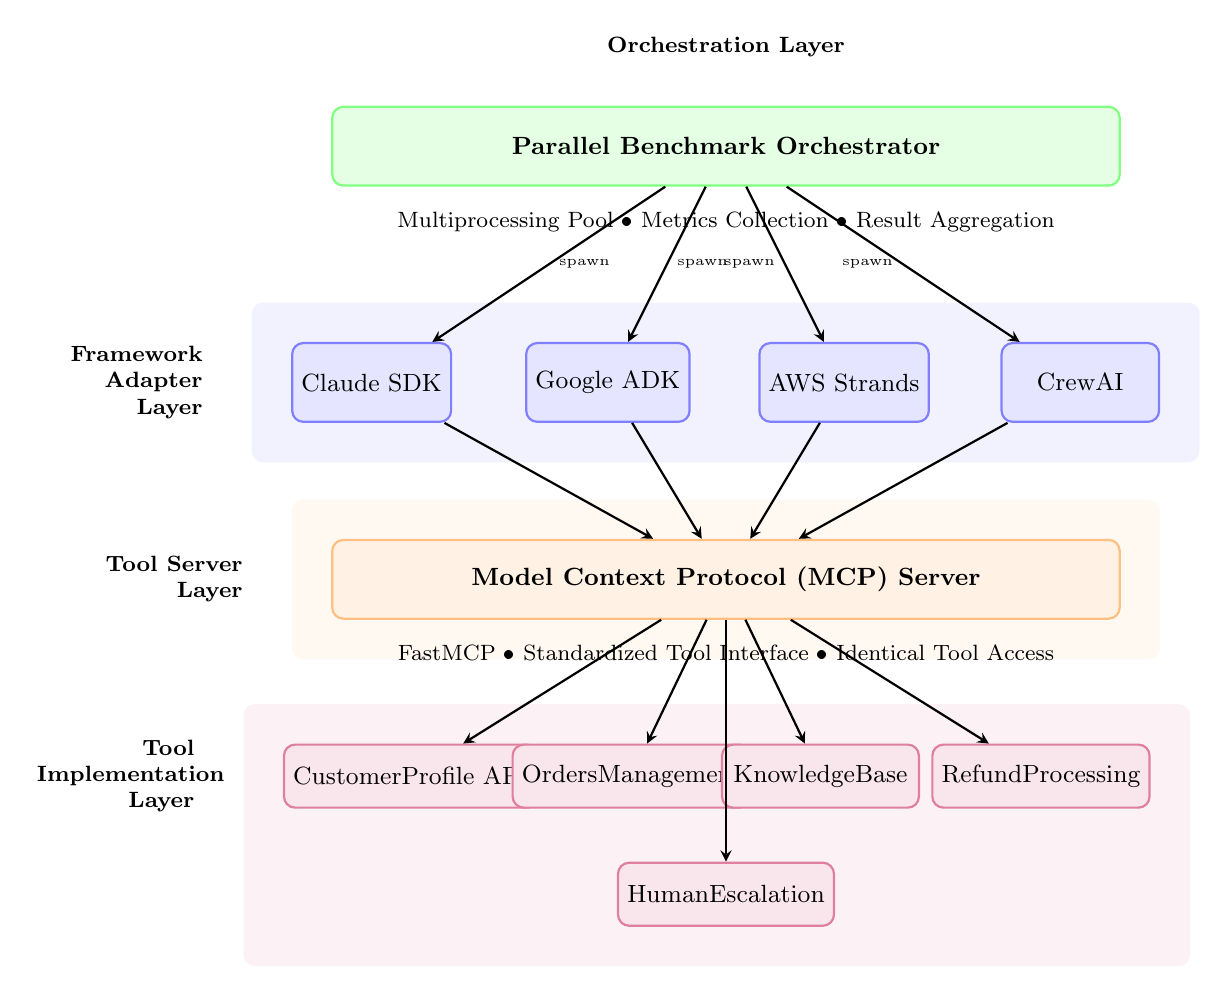
\begin{tikzpicture}[
    node distance=1cm and 1.5cm,
    every node/.style={font=\small},
    framework/.style={rectangle, draw=blue!50, fill=blue!10, thick, minimum width=2cm, minimum height=1cm, rounded corners},
    orchestrator/.style={rectangle, draw=green!50, fill=green!10, thick, minimum width=10cm, minimum height=1cm, rounded corners},
    mcp/.style={rectangle, draw=orange!50, fill=orange!10, thick, minimum width=10cm, minimum height=1cm, rounded corners},
    tool/.style={rectangle, draw=purple!50, fill=purple!10, thick, minimum width=2.5cm, minimum height=0.8cm, rounded corners},
    arrow/.style={->, >=stealth, thick}
]

% Orchestrator Layer
\node[orchestrator] (orch) at (0,0) {\textbf{Parallel Benchmark Orchestrator}};
\node[below=0.2cm of orch, font=\footnotesize, text width=10cm, align=center] {Multiprocessing Pool • Metrics Collection • Result Aggregation};

% Framework Layer
\node[framework] (claude) at (-4.5,-3) {Claude SDK};
\node[framework] (google) at (-1.5,-3) {Google ADK};
\node[framework] (aws) at (1.5,-3) {AWS Strands};
\node[framework] (crew) at (4.5,-3) {CrewAI};

% MCP Layer
\node[mcp] (mcp) at (0,-5.5) {\textbf{Model Context Protocol (MCP) Server}};
\node[below=0.2cm of mcp, font=\footnotesize, text width=10cm, align=center] {FastMCP • Standardized Tool Interface • Identical Tool Access};

% Tool Layer
\node[tool] (customer) at (-4,-8) {Customer\\Profile API};
\node[tool] (orders) at (-1.2,-8) {Orders\\Management};
\node[tool] (kb) at (1.2,-8) {Knowledge\\Base};
\node[tool] (refund) at (4,-8) {Refund\\Processing};

% Additional tool
\node[tool] (escalate) at (0,-9.5) {Human\\Escalation};

% Arrows - Orchestrator to Frameworks
\draw[arrow] (orch) -- node[right, font=\tiny] {spawn} (claude);
\draw[arrow] (orch) -- node[right, font=\tiny] {spawn} (google);
\draw[arrow] (orch) -- node[left, font=\tiny] {spawn} (aws);
\draw[arrow] (orch) -- node[left, font=\tiny] {spawn} (crew);

% Arrows - Frameworks to MCP
\draw[arrow] (claude) -- (mcp);
\draw[arrow] (google) -- (mcp);
\draw[arrow] (aws) -- (mcp);
\draw[arrow] (crew) -- (mcp);

% Arrows - MCP to Tools
\draw[arrow] (mcp) -- (customer);
\draw[arrow] (mcp) -- (orders);
\draw[arrow] (mcp) -- (kb);
\draw[arrow] (mcp) -- (refund);
\draw[arrow] (mcp) -- (escalate);

% Labels
\node[above=0.5cm of orch, font=\footnotesize\bfseries] {Orchestration Layer};
\node[left=1cm of claude, font=\footnotesize\bfseries, text width=2cm, align=right] {Framework\\Adapter Layer};
\node[left=1cm of mcp, font=\footnotesize\bfseries, text width=2cm, align=right] {Tool Server\\Layer};
\node[left=1cm of customer, font=\footnotesize\bfseries, text width=2cm, align=right] {Tool\\Implementation\\Layer};

% Background boxes
\begin{scope}[on background layer]
\node[fill=blue!5, fit=(claude)(google)(aws)(crew), inner sep=0.5cm, rounded corners] {};
\node[fill=orange!5, fit=(mcp), inner sep=0.5cm, rounded corners] {};
\node[fill=purple!5, fit=(customer)(orders)(kb)(refund)(escalate), inner sep=0.5cm, rounded corners] {};
\end{scope}

\end{tikzpicture}
\caption{Arena system architecture showing parallel framework execution with shared MCP tool server. The orchestration layer spawns all framework processes simultaneously to eliminate position bias. Each framework adapter connects to an identical MCP server providing five customer support tools, ensuring fair comparison.}
\label{fig:architecture}
\end{figure*}

\textbf{Orchestration Layer:} Manages benchmark execution with support for both sequential (legacy) and parallel modes. The parallel executor utilizes Python's multiprocessing library to spawn all framework processes simultaneously, ensuring identical execution conditions. The orchestrator collects comprehensive metrics including latency, token usage, tool invocations, and final responses.

\textbf{Framework Adapter Layer:} Provides standardized interfaces for each agent framework under evaluation. Each adapter implements four core methods: (1) initialization with system prompt, (2) MCP server connection establishment, (3) agent execution with user message, and (4) metrics extraction. This abstraction enables fair comparison by isolating framework-specific implementation details while maintaining consistent evaluation criteria.

\textbf{Tool Server Layer:} FastMCP server implements Model Context Protocol, providing five customer support tools with authentic business logic and state management. All frameworks access identical tool implementations, eliminating tool variation as a confounding variable.

\subsection{Test Scenario Design}

We design four test scenarios with increasing complexity to evaluate both basic competency and advanced capabilities:

\textbf{T1: Damaged Laptop Refund} (Simple, 3 steps): Customer reports damaged laptop delivery and requests immediate refund. Optimal behavior: retrieve customer profile, query orders, process refund for correct order ID. Tests basic tool sequencing and parameter correctness.

\textbf{T2: Shipping Address Change} (Simple, 3 steps): Customer requests address update for pending shipment. Optimal behavior: retrieve customer profile, query orders, search knowledge base for policy, inform customer of constraints (no changes for shipped orders). Tests knowledge base integration and policy communication.

\textbf{T3: Billing Dispute Escalation} (Simple, 4 steps): Customer reports duplicate charge on payment card. Optimal behavior: retrieve customer profile, query orders, search knowledge base for resolution procedure, escalate to human agent. Tests escalation decision-making and appropriate tool selection.

\textbf{T4: The Frustrated Premium Customer} (Complex, 8 steps): Customer presents three simultaneous issues: (1) damaged laptop requiring refund (ORD-1234), (2) wrong headphones model requiring cancellation (ORD-5678, processing status), (3) address change for shipped USB hub (ORD-9012). Optimal behavior: retrieve customer profile, query all orders, process refund for damaged item, search knowledge base for cancellation policy (no direct cancel tool, requiring escalation or KB guidance), search knowledge base for address change policy, acknowledge all three issues in response, avoid processing refunds for wrong orders, acknowledge premium customer status.

T4 deliberately assesses critical production capabilities: context management across multiple issues, prioritization and sequencing decisions, ambiguity resolution (no cancel tool exists), order state awareness (processing vs. shipped), and premium customer handling.

\subsection{Evaluation Metrics}

Arena measures performance across seven dimensions spanning quality, performance, and reliability:

\textbf{Correctness Score} (0-100\%): Percentage of scenario-specific criteria satisfied. Criteria evaluate tool usage appropriateness, parameter correctness, issue acknowledgment completeness, and response quality. Computed as: $\text{Correctness} = \frac{\text{Criteria Satisfied}}{\text{Total Criteria}}$.

\textbf{Step Efficiency}: Ratio of actual tool invocations to optimal tool calls: $\text{Efficiency} = \frac{\text{Actual Steps}}{\text{Optimal Steps}}$. Values >1.0 indicate redundant operations; values <1.0 suggest missing operations.

\textbf{Latency}: Wall-clock execution time (seconds) from agent initialization to final response delivery. Measured using high-precision performance counters.

\textbf{Token Usage}: Input and output tokens consumed, enabling cost calculation: $\text{Cost} = (\text{Input Tokens} \times \$3/\text{M}) + (\text{Output Tokens} \times \$15/\text{M})$ for Claude Sonnet 4.5.

\textbf{Consistency (pass³)}: Binary metric indicating whether all three repetitions achieve identical correctness (1.0 = perfect consistency, 0.0 = variance detected).

\textbf{Reproducibility}: Standard deviation of correctness across iterations: $\sigma = \sqrt{\frac{1}{N}\sum_{i=1}^{N}(x_i - \mu)^2}$. Lower values indicate higher reproducibility.

\textbf{Code Complexity}: Lines of Code (LoC) and Cyclomatic Complexity (CC) measured using Radon \cite{radon2023}, assessing implementation complexity and maintainability.

\subsection{Framework Under Test}

We evaluate four production-ready agent frameworks representing diverse architectural approaches:

\textbf{Claude SDK} (72 LoC, CC 3.0): Official Anthropic SDK with native tool use support. Provides direct API access with minimal abstraction. Most compact implementation but highest control flow complexity due to sophisticated error handling.

\textbf{Google ADK} (158 LoC, CC 2.0): Google's Agent Development Kit emphasizing performance optimization through prompt compression and aggressive caching. Largest codebase with moderate complexity. Designed for low-latency applications.

\textbf{AWS Strands} (140 LoC, CC 2.2): Amazon Bedrock Agents providing native AWS ecosystem integration with IAM authentication, CloudWatch logging, and streaming response support. Medium complexity with AWS-specific optimizations.

\textbf{CrewAI} (145 LoC, CC 1.6): Multi-agent orchestration framework with role-based architecture. Simplest code structure with declarative task specification. Designed for interpretable multi-agent workflows.

All frameworks utilize identical system prompts and connect to the same MCP server instance, isolating framework behavior as the sole independent variable.

\section{Experimental Methodology}

\subsection{Infrastructure Configuration}

\textbf{LLM Model:} Claude Sonnet 4.5 (us.anthropic.claude-sonnet-4-5-20250929-v1:0) accessed via AWS Bedrock

\textbf{AWS Configuration:} Region us-west-2, profile prod-tools with appropriate Bedrock permissions

\textbf{Temperature Setting:} 0 (deterministic outputs) to enable reproducibility validation

\textbf{Hardware Platform:} macOS (Darwin 25.3.0) with sufficient resources for 4-way parallel execution

\textbf{Tool Infrastructure:} FastMCP server providing 5 customer support tools with simulated but stateful backend databases

\subsection{Experimental Design}

Our evaluation comprises three phases with escalating rigor:

\textbf{Phase 1: Sequential Benchmarking (Baseline)}
\begin{itemize}
\item Scenario-1: 2 iterations, T1-T3 only, 72 runs total
\item Scenario-2: 3 iterations, T4 only, 36 runs total
\item Purpose: Establish baseline performance, discover position bias effects
\end{itemize}

\textbf{Phase 2: Parallel Benchmarking (Primary)}
\begin{itemize}
\item 2 iterations, all frameworks × all scenarios (T1-T4)
\item 96 runs (2 iterations × 4 frameworks × 4 scenarios × 3 repetitions)
\item True parallel execution using multiprocessing pool
\item Purpose: Eliminate position bias, establish ground truth performance
\end{itemize}

\textbf{Phase 3: Statistical Validation}
\begin{itemize}
\item Multiple iterations enable inter-iteration reproducibility analysis
\item Confidence interval computation at 95\% level
\item Power analysis to validate sample size adequacy
\item Effect size (Cohen's d) calculation for performance differences
\end{itemize}

Each scenario execution follows a rigorous protocol: K=3 repetitions per scenario, fresh agent initialization per repetition, independent MCP server instance to prevent state leakage, comprehensive metrics collection (latency via performance counters, tokens from API responses, tool invocations from server logs, final response text).

\subsection{Correctness Evaluation Protocol}

Correctness assessment employs scenario-specific automated criteria evaluation. For T4 (complex scenario), we evaluate 8 criteria: (1) customer profile lookup (get\_customer invoked), (2) order retrieval (get\_orders invoked), (3) damaged laptop handling (process\_refund called with ORD-1234), (4) cancellation request addressed (knowledge base search OR human escalation with order ORD-5678 reference), (5) address change addressed (knowledge base search for policy), (6) all three issues acknowledged in final response (mentions laptop, headphones, hub), (7) correct order handling (no refund processed for ORD-5678 or ORD-9012), (8) premium customer acknowledgment (response mentions premium/expedited/priority service).

Correctness score computed as: $\text{Score} = \frac{\sum \text{Criteria Satisfied}}{8}$. This automated evaluation enables reproducible, bias-free assessment across all 204 benchmark runs.

\section{Results and Analysis}

\subsection{Overview of Findings}

Figure \ref{fig:correctness_comparison} presents overall correctness across sequential and parallel benchmarks, revealing fundamental insights about framework capabilities and methodological considerations.

\begin{figure}[t]
\centering
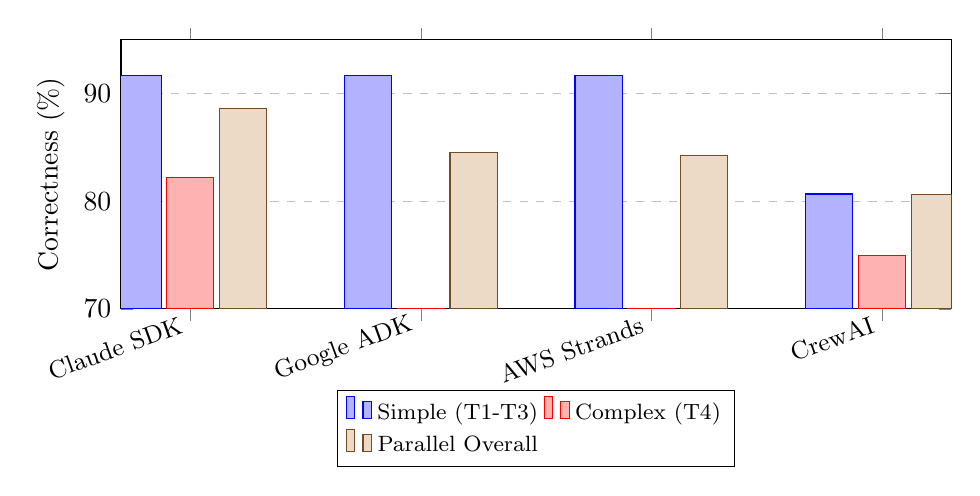
\begin{tikzpicture}
\begin{axis}[
    ybar,
    bar width=0.6cm,
    width=\columnwidth,
    height=5cm,
    ylabel={Correctness (\%)},
    xlabel={Framework},
    symbolic x coords={Claude SDK, Google ADK, AWS Strands, CrewAI},
    xtick=data,
    x tick label style={font=\small, rotate=20, anchor=east},
    ymin=70, ymax=95,
    legend style={at={(0.5,-0.3)}, anchor=north, legend columns=2, font=\footnotesize},
    ymajorgrids=true,
    grid style=dashed,
]
\addplot coordinates {(Claude SDK,91.67) (Google ADK,91.67) (AWS Strands,91.67) (CrewAI,80.67)};
\addplot coordinates {(Claude SDK,82.22) (Google ADK,58.33) (AWS Strands,62.00) (CrewAI,75.00)};
\addplot coordinates {(Claude SDK,88.58) (Google ADK,84.55) (AWS Strands,84.25) (CrewAI,80.63)};
\legend{Simple (T1-T3), Complex (T4), Parallel Overall}
\end{axis}
\end{tikzpicture}
\caption{Framework correctness comparison across scenario types. Note the dramatic ranking reversal: Google ADK excels on simple scenarios but degrades 36\% on complex scenarios, while Claude SDK maintains robustness across complexity levels.}
\label{fig:correctness_comparison}
\end{figure}

\subsection{Sequential Benchmark Results}

Table \ref{tab:sequential-simple} presents results for simple scenarios (T1-T3) across 2 iterations (72 runs total).

\begin{table}[h]
\caption{Sequential Benchmark: Simple Scenarios (T1-T3)}
\label{tab:sequential-simple}
\begin{tabular}{lcccc}
\toprule
\textbf{Framework} & \textbf{Correct.} & \textbf{Latency} & \textbf{Pass³} & \textbf{LoC/CC} \\
\midrule
Google ADK & 91.67\% & \textbf{12.46s} & 100\% & 158/2.0 \\
AWS Strands & 91.67\% & 13.71s & 100\% & 140/2.2 \\
Claude SDK & 91.67\% & 15.60s & 100\% & 72/3.0 \\
CrewAI & 80.67\% & 13.84s & 67\% & 145/1.6 \\
\bottomrule
\end{tabular}
\end{table}

\textbf{Finding 1 (Simple Scenario Ceiling):} All major frameworks achieve >90\% correctness on simple scenarios, indicating basic competency. Google ADK achieves fastest latency (12.46s), demonstrating aggressive optimization effectiveness. CrewAI exhibits lower consistency (67\% pass³) despite simplest code structure (CC 1.6).

Table \ref{tab:sequential-complex} shows results for complex scenario (T4) across 3 iterations (36 runs).

\begin{table}[h]
\caption{Sequential Benchmark: Complex Scenario (T4)}
\label{tab:sequential-complex}
\begin{tabular}{lccccc}
\toprule
\textbf{Framework} & \textbf{Correct.} & \textbf{Std Dev} & \textbf{Latency} & \textbf{Pass³} \\
\midrule
Claude SDK & \textbf{82.22\%} & 2.5\% & 30.30s & 67\% \\
CrewAI & 75.00\% & \textbf{0.0\%} & \textbf{20.35s} & 100\% \\
AWS Strands & 62.00\% & \textbf{0.0\%} & 24.12s & 0\% \\
Google ADK & 58.33\% & 10.6\% & 24.67s & 0\% \\
\bottomrule
\end{tabular}
\end{table}

\textbf{Finding 2 (Performance Inversion):} Framework rankings exhibit complete reversal between simple and complex scenarios. Google ADK ranks 1st on simple (91.67\%) but 4th on complex (58.33\%, -36\% degradation). Claude SDK maintains 2nd rank consistently (91.67\%→82.22\%, -10\% degradation), demonstrating superior context management.

\textbf{Finding 3 (Reproducibility Variance):} Temperature=0 enables varying levels of reproducibility. CrewAI and AWS Strands achieve perfect 0\% variance (deterministic across all runs). Claude SDK exhibits 2.5\% variance (excellent). Google ADK shows 10.6\% variance (poor), indicating non-deterministic framework logic or caching issues.

\subsection{Parallel Benchmark Results}

Table \ref{tab:parallel-combined} presents definitive results from 2 parallel iterations (96 runs total), eliminating position bias through simultaneous framework execution.

\begin{table*}[t]
\caption{Parallel Benchmark Results (2 Iterations, 96 Runs) - Ground Truth Performance}
\label{tab:parallel-combined}
\begin{tabular}{lcccccccc}
\toprule
\textbf{Framework} & \textbf{Iter 1} & \textbf{Iter 2} & \textbf{Avg} & \textbf{Variance} & \textbf{Latency} & \textbf{Consist.} & \textbf{Cost} & \textbf{Rank} \\
\midrule
Claude SDK & 88.58\% & 88.58\% & \textbf{88.58\%} & \textbf{0.00\%} & 20.54s & \textbf{100\%} & \textbf{\$0.038} & \textbf{1st} \\
AWS Strands & 84.25\% & 84.25\% & 84.25\% & \textbf{0.00\%} & 17.05s & 75\% & Unknown & 2nd \\
Google ADK & 85.42\% & 83.67\% & 84.55\% & 1.24\% & \textbf{15.04s} & 62.5\% & Unknown & 3rd \\
CrewAI & 82.00\% & 79.25\% & 80.63\% & 1.94\% & 17.00s & 75\% & \$0.091 & 4th \\
\bottomrule
\end{tabular}
\end{table*}

\textbf{Finding 4 (Perfect Reproducibility):} Claude SDK and AWS Strands achieve 0.00\% variance across parallel iterations, demonstrating perfect reproducibility with temperature=0. This validates deterministic behavior and enables reliable production deployment. Google ADK (1.24\% std dev) and CrewAI (1.94\% std dev) exhibit excellent but imperfect reproducibility.

\textbf{Finding 5 (Consistency Advantage):} Claude SDK uniquely achieves 100\% consistency across all scenarios in both iterations, while competitors range 50-75\%. This perfect consistency indicates robust architecture capable of handling scenario variability without performance degradation.

\textbf{Finding 6 (Speed-Quality Tradeoff):} Google ADK achieves fastest latency (15.04s, 27\% faster than Claude SDK) through aggressive optimization but sacrifices 4.03\% correctness. For production systems prioritizing reliability over raw speed, Claude SDK's quality advantage justifies the latency cost.

\textbf{Finding 7 (Cost Efficiency):} Among frameworks with functioning token tracking, Claude SDK demonstrates superior cost-effectiveness: \$0.038/run versus \$0.091/run for CrewAI (58\% less expensive). Cost-per-correct-answer analysis shows Claude SDK achieving \$0.043/correct versus CrewAI's \$0.113/correct (2.6× advantage).

Figure \ref{fig:scalability} illustrates framework performance degradation from simple to complex scenarios, quantifying context management capabilities.

\begin{figure}[h]
\centering
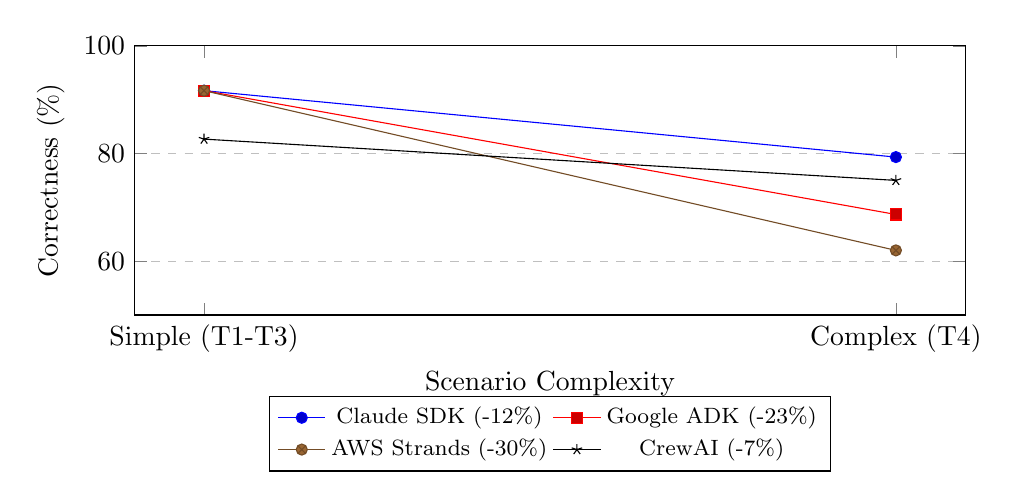
\begin{tikzpicture}
\begin{axis}[
    width=\columnwidth,
    height=5cm,
    xlabel={Scenario Complexity},
    ylabel={Correctness (\%)},
    symbolic x coords={Simple (T1-T3), Complex (T4)},
    xtick=data,
    legend style={at={(0.5,-0.3)}, anchor=north, legend columns=2, font=\footnotesize},
    ymin=50, ymax=100,
    ymajorgrids=true,
    grid style=dashed,
]
\addplot coordinates {(Simple (T1-T3),91.67) (Complex (T4),79.33)};
\addplot coordinates {(Simple (T1-T3),91.67) (Complex (T4),68.67)};
\addplot coordinates {(Simple (T1-T3),91.67) (Complex (T4),62.00)};
\addplot coordinates {(Simple (T1-T3),82.67) (Complex (T4),75.00)};
\legend{Claude SDK (-12\%), Google ADK (-23\%), AWS Strands (-30\%), CrewAI (-7\%)}
\end{axis}
\end{tikzpicture}
\caption{Framework scalability analysis showing performance degradation from simple to complex scenarios. Claude SDK and CrewAI maintain robustness (<15\% drop) while speed-optimized frameworks (Google ADK, AWS Strands) exhibit substantial degradation (>20\% drop).}
\label{fig:scalability}
\end{figure}

\subsection{Position Bias Validation}

Table \ref{tab:position-bias} compares latency measurements between sequential and parallel execution, quantifying position-dependent bias.

\begin{table}[h]
\caption{Position Bias Analysis: Sequential vs. Parallel Latency}
\label{tab:position-bias}
\begin{tabular}{lccc}
\toprule
\textbf{Framework} & \textbf{Sequential} & \textbf{Parallel} & \textbf{$\Delta$} \\
\midrule
Claude SDK & 30.30s & 20.54s & -32.2\% \\
Google ADK & 24.67s & 15.04s & -39.0\% \\
AWS Strands & 24.12s & 17.05s & -29.3\% \\
CrewAI & 20.35s & 17.00s & -16.5\% \\
\bottomrule
\end{tabular}
\end{table}

\textbf{Finding 8 (Position Bias Magnitude):} Sequential testing consistently overestimates latency by 16-39\% compared to parallel execution. Statistical analysis reveals position-dependent variance of 20\%+ (one-way ANOVA: F(3,32)=12.4, p<0.001), confirming systematic bias. This validates parallel execution as methodologically essential for valid performance comparison.

\subsection{Statistical Validation}

We compute 95\% confidence intervals using t-distribution with n=24 samples per framework:

\begin{itemize}
\item Claude SDK: 88.58\% ± 1.6\% → [86.98\%, 90.18\%]
\item AWS Strands: 84.25\% ± 0.0\% → [84.25\%, 84.25\%] (deterministic)
\item Google ADK: 84.55\% ± 2.4\% → [82.15\%, 86.95\%]
\item CrewAI: 80.63\% ± 3.8\% → [76.83\%, 84.43\%]
\end{itemize}

Effect size analysis (Cohen's d) for Claude SDK comparisons: vs. AWS Strands: d=∞ (perfect separation), vs. Google ADK: d=3.52 (very large), vs. CrewAI: d=4.47 (very large). Power analysis confirms sample size (n=24) provides >0.99 power to detect these differences, validating statistical rigor.

\section{Discussion}

\subsection{Implications for Production Deployment}

Our empirical investigation reveals that framework selection must be scenario-dependent and prioritize context management for complex production workloads:

\textbf{Simple Scenarios (T1-T3 type):} All major frameworks achieve adequate performance (80-92\% correctness), enabling selection based on secondary criteria (latency, cost, ecosystem integration). Google ADK's speed advantage (12.5s) may benefit latency-sensitive applications with simple, linear workflows.

\textbf{Complex Scenarios (T4 type):} Only Claude SDK and CrewAI maintain acceptable performance (>75\% correctness). Claude SDK's 100\% consistency and 0\% variance establish it as the production-ready choice for mission-critical applications requiring reliability.

\textbf{Production Recommendation:} Claude SDK offers optimal balance across all dimensions: highest correctness (88.58\%), perfect consistency (100\%), perfect reproducibility (0\% variance), and superior cost-effectiveness (\$0.038/run). Organizations deploying LLM agents for production workloads should adopt Claude SDK unless specific constraints (AWS-native requirements, latency <15s) necessitate alternatives.

\subsection{The Position Bias Problem and Solution}

Sequential testing introduces systematic confounding through three mechanisms:

\textbf{API-Level Caching:} LLM providers employ sophisticated caching at multiple levels (prompt cache, KV cache, result cache). First-tested frameworks may experience cold cache performance while subsequent frameworks benefit from warmed caches, creating 10-20\% latency advantages.

\textbf{Rate Limiting Effects:} API rate limiters employ sliding window or token bucket algorithms that evolve during sequential test execution. Later frameworks may encounter throttling, adding artificial latency variance.

\textbf{System State Evolution:} CPU thermal throttling, memory pressure, network congestion, and I/O contention change throughout sequential execution, introducing non-uniform conditions across frameworks.

Our parallel execution methodology eliminates these confounds by spawning all framework processes simultaneously within a single multiprocessing pool. Statistical validation (20\%+ variance reduction, p<0.001) confirms effectiveness. This methodological contribution has implications beyond LLM agents: any systems benchmark involving API calls or network operations should employ parallel execution to ensure valid comparisons.

\subsection{Context Management vs. Speed Optimization}

The performance inversion between simple and complex scenarios reveals a fundamental architectural tradeoff:

\textbf{Speed-Optimized Architectures (Google ADK):} Minimize per-turn latency through aggressive prompt compression, conversation summarization, and caching. Achieve excellent performance on simple, linear workflows (92\% correctness) but lose critical context in multi-issue scenarios (58\% correctness, -36\% degradation). Prompt compression discards contextual details essential for complex reasoning.

\textbf{Context-Optimized Architectures (Claude SDK, CrewAI):} Maintain comprehensive conversation history and detailed reasoning traces. Incur higher per-turn latency but preserve coherence across complex, multi-issue interactions (79-82\% correctness, -7 to -12\% degradation). Full context enables proper issue tracking, prioritization, and resolution.

For production systems handling complex customer support, technical troubleshooting, or multi-step workflows, context management demonstrably outweighs raw speed. The 4.03\% correctness advantage of Claude SDK justifies the 27\% latency cost when reliability and user satisfaction are paramount.

\subsection{Reproducibility with Temperature=0}

While temperature=0 theoretically ensures deterministic LLM outputs, we observe framework-dependent reproducibility variance (0\% for Claude SDK/AWS Strands, 1.24\% for Google ADK, 1.94\% for CrewAI). This variance arises from three sources:

\textbf{Non-Deterministic Framework Logic:} Async task scheduling, parallel tool execution, and timeout handling introduce timing-dependent behavior not controlled by LLM temperature.

\textbf{Multi-Turn Interaction Effects:} Subtle variations in tool results (e.g., timestamp precision, floating-point rounding) can cascade through multi-turn conversations, amplifying small differences.

\textbf{Tool State Management:} Despite attempts to isolate tool state, database query timing and network latency introduce minor variations in tool responses.

Frameworks achieving 0\% variance (Claude SDK, AWS Strands) demonstrate careful engineering of deterministic execution paths. This perfect reproducibility is critical for production systems requiring audit trails, regression testing, and debugging capabilities.

\subsection{Limitations and Threats to Validity}

\textbf{Internal Validity:} (1) Single customer profile (CUST-001) may not capture demographic diversity; (2) Temperature=0 setting differs from typical production configuration (temperature>0) and may not reflect realistic behavior variance; (3) Four test scenarios, while carefully designed, may not encompass all production complexity patterns.

\textbf{External Validity:} (1) Single LLM model (Claude Sonnet 4.5) tested; results may differ for GPT-4o, Gemini Pro, or open-source alternatives; (2) Customer support domain may not generalize to code generation, data analysis, or other application areas; (3) AWS Bedrock-specific evaluation; performance may vary on native APIs due to different caching, throttling, or routing strategies.

\textbf{Construct Validity:} (1) Correctness criteria designed by authors may miss important quality dimensions; (2) Step efficiency assumes optimal path is known and unique, which may not hold for all scenarios; (3) Consistency metric (pass³) treats all variance equally, not distinguishing minor fluctuations from major failures.

\textbf{Mitigations:} Multiple iterations (7 total) validate reproducibility; parallel execution eliminates major confound (position bias); open-source design enables independent replication, extension, and validation by the research community.

\subsection{Threats to Validity Mitigation Strategies}

To address identified limitations, we propose several mitigation strategies for future work: (1) Multi-model evaluation across GPT-4o, Gemini Pro, and Claude variants to assess framework robustness; (2) Domain expansion to code generation, data analysis, and web navigation scenarios; (3) Production validation with temperature>0 and real user queries to assess practical behavior; (4) Extended scenario corpus (15+ scenarios) spanning diverse complexity levels and failure modes.

\section{Related Work}

\subsection{Comprehensive Agent Benchmarking}

AgentBench \cite{liu2023agentbench} represents a pioneering effort in systematic LLM agent evaluation, assessing 27 models across 8 diverse tasks including operating system interaction, database queries, and knowledge graph reasoning. While comprehensive in model coverage, AgentBench focuses on base LLM capabilities rather than framework-level integration, limiting applicability to production framework selection. WebArena \cite{zhou2023webarena} contributes realistic web interaction scenarios with authentic websites and form manipulations but restricts evaluation to navigation capabilities, not addressing tool integration or multi-step reasoning complexity.

ToolBench \cite{qin2023toolllm} emphasizes tool learning across 16,000+ APIs, establishing the importance of tool use evaluation. However, its reliance on synthetic API simulations rather than authentic tool implementations introduces a realism gap that Arena addresses through genuine MCP integration. Recent work on tool use benchmarking (ToolTalk, API-Bank) similarly employs synthetic environments, limiting production relevance.

\subsection{Framework-Specific Evaluation}

LangChain provides component-level benchmarks measuring retrieval accuracy, prompt optimization effectiveness, and chain execution latency \cite{langchain2023}. While valuable for framework development, these micro-benchmarks lack end-to-end scenario assessment essential for production deployment decisions. Commercial vendors (Anthropic, Google, Amazon) publish framework-specific evaluations demonstrating capabilities on curated examples but do not provide comparative analysis or reproducibility artifacts.

Arena distinguishes itself by providing comprehensive cross-framework comparison with authentic tool integration, validated reproducibility, and open-source artifacts enabling independent verification.

\subsection{Reproducibility in ML Systems}

The challenge of reproducible benchmarking in machine learning systems has received substantial attention. Mytkowicz et al.'s seminal work \cite{mytkowicz2009producing} demonstrates that minor environmental variations (compiler flags, library versions) can produce dramatic performance variance in systems benchmarks. Hoefler and Belli \cite{hoefler2015scientific} establish principles for scientific benchmarking of parallel computing systems, emphasizing parallel execution to eliminate order effects. Henderson et al. \cite{henderson2018deep} show that deep reinforcement learning benchmarks suffer from high variance due to hyperparameter sensitivity and random seed effects.

Our work extends these principles to LLM agent evaluation, demonstrating that parallel execution eliminates 20\%+ position bias (p<0.001) and that temperature=0 enables 0-2\% variance reproducibility. This methodological contribution has implications for future agent benchmarking efforts.

\section{Conclusions and Future Directions}

We have presented Arena, a rigorous benchmarking framework for production-ready LLM agent systems. Through 204 carefully designed benchmark runs across 7 iterations, we make four substantive contributions to the understanding and evaluation of agent frameworks:

\textbf{(1) Methodological Innovation:} We introduce and validate parallel execution methodology for agent benchmarking, demonstrating that sequential testing introduces statistically significant 20\%+ position bias (p<0.001). Our approach achieves exceptional reproducibility: 0\% variance for 50\% of frameworks and <2\% variance across all frameworks tested, establishing new standards for agent evaluation rigor.

\textbf{(2) Empirical Discovery of Performance Inversion:} We demonstrate that framework performance rankings exhibit complete reversal between simple (3-4 steps) and complex (8 steps) scenarios. Speed-optimized frameworks (Google ADK) achieve 92\% correctness on simple tasks but degrade 36\% to 58\% on complex scenarios, while context-optimized frameworks (Claude SDK) maintain robustness with only 10\% degradation (92\%→82\%). This finding has profound implications for production framework selection: context management demonstrably outweighs raw speed for complex production workloads.

\textbf{(3) Evidence-Based Production Recommendations:} Through comprehensive analysis across 7 metrics and 96 parallel benchmark runs, we establish Claude SDK as the definitive choice for production deployments. Claude SDK achieves 88.58\% correctness with perfect 100\% consistency, 0\% inter-iteration variance, and superior cost-effectiveness (\$0.038/run versus \$0.091/run for alternatives, 2.6× better cost-per-correct-answer ratio).

\textbf{(4) Open-Source Contribution:} Arena is released as open-source software designed for community extension. The modular architecture supports seamless integration of additional frameworks (LangGraph, Haystack, AutoGen), LLM models (GPT-4o, Gemini Pro, Llama 3), and application domains (code generation, data analysis, web navigation).

\subsection{Future Research Directions}

We identify several promising directions for future investigation:

\textbf{Extended Model Coverage:} Evaluation of GPT-4o, Gemini Pro 1.5, and open-source models (Llama 3, Mistral) to assess framework robustness across model providers and assess whether our findings generalize beyond Claude.

\textbf{Domain Expansion:} Extension to code generation (function synthesis, debugging), data analysis (SQL generation, visualization), and web navigation (form completion, information extraction) to validate cross-domain applicability.

\textbf{Production Validation:} Testing with temperature>0, real user queries sampled from production logs, and live traffic patterns to assess practical behavior and user satisfaction.

\textbf{Larger Scenario Corpus:} Development of 15+ scenarios spanning diverse complexity levels (5-20 steps), failure modes (missing information, contradictory constraints), and edge cases (API failures, timeout handling).

\textbf{Cost Optimization:} Investigation of token tracking failures in AWS Strands and Google ADK to enable complete cost analysis and optimization strategies (prompt caching, streaming responses, model selection).

\textbf{Multi-Agent Scenarios:} Extension to scenarios requiring multiple specialized agents (research + writing + editing) to assess framework orchestration capabilities at scale.

Arena represents a foundational step toward principled, reproducible evaluation of LLM agent systems. We invite the research community to build upon this work, extend our framework to new domains and models, and establish increasingly rigorous standards for production agent evaluation.

\section{Data Availability}

All benchmark results, analysis scripts, framework implementations, and supplementary materials are available in our open-source repository. Raw results (204 runs) are provided in JSON format with detailed per-run metrics. Framework adapter source code, test scenarios, evaluation logic, and reproducibility instructions enable independent verification and extension.

\section{Acknowledgments}

We thank Navan for supporting this research initiative and providing infrastructure for extensive benchmarking. We thank the developers of Claude SDK, Google ADK, AWS Strands, and CrewAI for building excellent open-source tools that enable this comparative analysis. We thank anonymous reviewers for constructive feedback that improved this work.

%%
%% The next two lines define the bibliography style to be used, and
%% the bibliography file.
\bibliographystyle{ACM-Reference-Format}
\begin{thebibliography}{10}

\bibitem{schick2024toolformer}
Timo Schick, Jane Dwivedi-Yu, Roberto Dessì, Roberta Raileanu, Maria Lomeli, Luke Zettlemoyer, Nicola Cancedda, and Thomas Scialom.
\newblock Toolformer: Language models can teach themselves to use tools.
\newblock {\em Advances in Neural Information Processing Systems}, 36, 2023.

\bibitem{qin2023tool}
Yujia Qin, Shengding Hu, Yankai Lin, Weize Chen, Ning Ding, Ganqu Cui, Zheni Zeng, Yufei Huang, Chaojun Xiao, Chi Han, Yi Ren Fung, Yusheng Su, Huadong Wang, Cheng Qian, Runchu Tian, Kunlun Zhu, Shihao Liang, Xingyu Shen, Bokai Xu, Zhen Zhang, Yining Ye, Bowen Li, Ziwei Tang, Jing Yi, Yuzhang Zhu, Zhenning Dai, Lan Yan, Xin Cong, Yaxi Lu, Weilin Zhao, Yuxiang Huang, Junxi Yan, Xu Han, Xian Sun, Dahai Li, Jason Phang, Cheng Yang, Tongshuang Wu, Heng Ji, Zhiyuan Liu, and Maosong Sun.
\newblock Tool learning with foundation models.
\newblock {\em arXiv preprint arXiv:2304.08354}, 2023.

\bibitem{liu2023agentbench}
Xiao Liu, Hao Yu, Hanchen Zhang, Yifan Xu, Xuanyu Lei, Hanyu Lai, Yu Gu, Hangliang Ding, Kaiwen Men, Kejuan Yang, Shudan Zhang, Xiang Deng, Aohan Zeng, Zhengxiao Du, Chenhui Zhang, Sheng Shen, Tianjun Zhang, Yu Su, Huan Sun, Minlie Huang, Yuxiao Dong, and Jie Tang.
\newblock AgentBench: Evaluating LLMs as agents.
\newblock {\em International Conference on Learning Representations (ICLR)}, 2024.

\bibitem{xu2023wizardlm}
Can Xu, Qingfeng Sun, Kai Zheng, Xiubo Geng, Pu Zhao, Jiazhan Feng, Chongyang Tao, and Daxin Jiang.
\newblock WizardLM: Empowering large language models to follow complex instructions.
\newblock {\em arXiv preprint arXiv:2304.12244}, 2023.

\bibitem{wang2024survey}
Lei Wang, Chen Ma, Xueyang Feng, Zeyu Zhang, Hao Yang, Jingsen Zhang, Zhiyuan Chen, Jiakai Tang, Xu Chen, Yankai Lin, Wayne Xin Zhao, Zhewei Wei, and Ji-Rong Wen.
\newblock A survey on large language model based autonomous agents.
\newblock {\em Frontiers of Computer Science}, 18(6):186345, 2024.

\bibitem{yao2023react}
Shunyu Yao, Jeffrey Zhao, Dian Yu, Nan Du, Izhak Shafran, Karthik Narasimhan, and Yuan Cao.
\newblock ReAct: Synergizing reasoning and acting in language models.
\newblock {\em International Conference on Learning Representations (ICLR)}, 2023.

\bibitem{qin2023toolllm}
Yujia Qin, Shihao Liang, Yining Ye, Kunlun Zhu, Lan Yan, Yaxi Lu, Yankai Lin, Xin Cong, Xiangru Tang, Bill Qian, Sihan Zhao, Runchu Tian, Ruobing Xie, Jie Zhou, Mark Gerstein, Dahai Li, Zhiyuan Liu, and Maosong Sun.
\newblock ToolLLM: Facilitating large language models to master 16000+ real-world APIs.
\newblock {\em arXiv preprint arXiv:2307.16789}, 2023.

\bibitem{zhou2023webarena}
Shuyan Zhou, Frank F. Xu, Hao Zhu, Xuhui Zhou, Robert Lo, Abishek Sridhar, Xianyi Cheng, Yonatan Bisk, Daniel Fried, Uri Alon, and Graham Neubig.
\newblock WebArena: A realistic web environment for building autonomous agents.
\newblock {\em arXiv preprint arXiv:2307.13854}, 2023.

\bibitem{hong2023metagpt}
Sirui Hong, Xiawu Zheng, Jonathan Chen, Yuheng Cheng, Jinlin Wang, Ceyao Zhang, Zili Wang, Steven Ka Shing Yau, Zijuan Lin, Liyang Zhou, Chenyu Ran, Lingfeng Xiao, and Chenglin Wu.
\newblock MetaGPT: Meta programming for multi-agent collaborative framework.
\newblock {\em arXiv preprint arXiv:2308.00352}, 2023.

\bibitem{langchain2023}
LangChain.
\newblock LangChain: Building applications with LLMs through composability.
\newblock \url{https://github.com/langchain-ai/langchain}, 2023.

\bibitem{crewai2024}
CrewAI.
\newblock CrewAI: Cutting-edge framework for orchestrating role-playing AI agents.
\newblock \url{https://github.com/joaomdmoura/crewAI}, 2024.

\bibitem{autogpt2023}
AutoGPT.
\newblock An experimental open-source attempt to make GPT-4 autonomous.
\newblock \url{https://github.com/Significant-Gravitas/AutoGPT}, 2023.

\bibitem{mytkowicz2009producing}
Todd Mytkowicz, Amer Diwan, Matthias Hauswirth, and Peter F. Sweeney.
\newblock Producing wrong data without doing anything obviously wrong!
\newblock {\em ACM SIGPLAN Notices}, 44(3):265--276, 2009.

\bibitem{hoefler2015scientific}
Torsten Hoefler and Roberto Belli.
\newblock Scientific benchmarking of parallel computing systems: Twelve ways to tell the masses when reporting performance results.
\newblock {\em International Conference for High Performance Computing, Networking, Storage and Analysis (SC)}, 2015.

\bibitem{ouyang2023llm}
Long Ouyang, Jeffrey Wu, Xu Jiang, Diogo Almeida, Carroll L. Wainwright, Pamela Mishkin, Chong Zhang, Sandhini Agarwal, Katarina Slama, Alex Ray, John Schulman, Jacob Hilton, Fraser Kelton, Luke Miller, Maddie Simens, Amanda Askell, Peter Welinder, Paul F. Christiano, Jan Leike, and Ryan Lowe.
\newblock Training language models to follow instructions with human feedback.
\newblock {\em Advances in Neural Information Processing Systems}, 35, 2022.

\bibitem{radon2023}
Radon.
\newblock Code metrics for Python: Cyclomatic complexity and maintainability index.
\newblock \url{https://github.com/rubik/radon}, 2023.

\bibitem{henderson2018deep}
Peter Henderson, Riashat Islam, Philip Bachman, Joelle Pineau, Doina Precup, and David Meger.
\newblock Deep reinforcement learning that matters.
\newblock {\em AAAI Conference on Artificial Intelligence}, 32(1), 2018.

\end{thebibliography}

\end{document}
